% Mirror: https://github.com/SIGma-UIUC/presentation-format
% --------------------------------------------------------------------
% This is a simple Beamer document that uses beamerthemesigma.sty
% Reading the comments should help you create a presentation even if
% you've never used Beamer before.
% --------------------------------------------------------------------

% Set our document class to Beamer
\documentclass[aspectratio=169]{beamer}
% \documentclass[aspectratio=169, handout]{beamer}
% Add handout option to ignore pauses

% From Jeff E
\usepackage{algo}
% Some more macros
\usepackage{sigmastyle}

\definecolor{LightGreen}{RGB}{80,252,80}

% Set a title
\title{Burst Codes}

% Whoever worked on the presentation:
\author{Alex Broihier, Porter Shawver}

% Date looks ugly, so leave blank
\date{}

% An institute name, if you're so inclined
% \institute{University of Illinois Urbana-Champaign}

% Use the SIGma theme for this Beamer presentation
\usetheme{sigma}

\newcommand{\err}[1]{{\color{sigma@alertred}#1}}
\newcommand{\blu}[1]{{\color{sigma@mainblue}#1}}

\newcommand{\lgreen}[1]{{\color{LightGreen}#1}}
% --------------------------------------------------------------------

% Begin document
\begin{document}

% Beamer calls each slide a "frame", defined within the environment:
% \begin{frame}
%   <frame content here>
% \end{frame}

% This frame is just the title.
\begin{frame}
\titlepage
\end{frame}

% A frame with the table of contents.
% This frame's title is "Outline".
\begin{frame}{Outline}
  \tableofcontents
\end{frame}

\section{Cyclic Codes}
\frame{\sectionpage}

%%%%%%%%%%%%%%%%%%%%%%%%%%%%%%%%%%%%
%%%%%%%%%%% Burst Errors %%%%%%%%%%%
%%%%%%%%%%%%%%%%%%%%%%%%%%%%%%%%%%%%
\begin{frame}{Burst Errors}
    \begin{itemize}
        \item Burst Description $(P, L)$ where $P$ is the error, $L$ is the starting index
        \item $E = [0, 1, 1, 0, 0, 1]$ is the error in some message
        \item $(11001, 2)$ describes $E$ 
        \item More common in the real world (think scratching a CD, the internet dropping in the middle of a message, etc.)
    \end{itemize}
\end{frame}


%%%%%%%%%%%%%%%%%%%%%%%%%%%%%%%%%%%%
%%%%%%%%%%% CYCLIC CODES %%%%%%%%%%%
%%%%%%%%%%%%%%%%%%%%%%%%%%%%%%%%%%%%


\begin{frame}{What are Cyclic Codes}
    \begin{itemize}
        \item Invariant under rotation
        \begin{itemize}
            \item $011001$, $101100$, $010110$, $001011$, $100101$, $110010$ all the same
        \end{itemize}
        \item When considering cycles with burst errors, the burst description is no longer unique \pause
        \item $E = [0, 1, 1, 0, 0, 1]$ is described by $(11001, 2), (100101, 3), \text{ and } (1011, 6)$ \pause
        \item $E \xrightarrow[]{\text{Rotated To}} [1, 0, 0, 1, 0, 1]$ is described by $(1011, 4)$
        \item $E \xrightarrow[]{\text{Rotated To}} [1, 0, 1, 1, 0, 0]$ is described by $(100101, 4)$
    \end{itemize}
\end{frame}


\begin{frame}{Generating Functions for Linear Cyclic Codes}
    \begin{itemize}
        \item Coefficient of each term corresponds to a corresponding digit in code
        \item $g(x) = 1x^0 + 0x^1 + 1x^2 + 1x^3 + 0x^4$ corresponds to $10110$ \pause
        \item A multiplication by $x$ corresponds to a rotation:
        \begin{align*}
            x \cdot g(x)
            & = 1x^1 + 0x^2 + 1x^3 + 1x^4 + 0x^5 \\
            & = 1x^1 + 0x^2 + 1x^3 + 1x^4 + 0x^0 \\
            & = 0x^0 + 1x^1 + 0x^2 + 1x^3 + 1x^4 \\
            & \to 01011
        \end{align*}
    \end{itemize}
\end{frame}

\begin{frame}{Cyclic Codespace}
    Let $w$ be the original, un-encoded message.

    \begin{center}
        $w$ 
        \pause
        $\xrightarrow[]{\text{Encode}} w\cdot g(x)$
        \pause
        $\xrightarrow[]{\text{Transmission Error}} w \cdot g(x) + e(x)$
        \pause
        $\xrightarrow[]{\text{Mod } g(x)} e(x)$.
    \end{center}
    \pause
    \begin{itemize}
        \item $e(x)$ obtained as remainder when dividing by $g(x)$
    \end{itemize}
\end{frame}

\begin{frame}{Example}
    \begin{itemize}
        \item Say we want to encode $\{00, 10, 01, 11\}$
        \item Let's pick $g(x) = 1 + x^2$ as our generator
    \end{itemize} \pause

    \bigskip

    \begin{columns}[c]
    \begin{column}{3cm}
        $\quad 00$
    \end{column}
    \begin{column}{3cm}
        $10$
    \end{column}
    \begin{column}{3cm}
        $01$
    \end{column}
    \begin{column}{3cm}
        $11$
    \end{column}
    \hfill
    \end{columns} \pause

    \begin{columns}[c]
    \begin{column}{3cm}
        $\to 0$
    \end{column}
    \begin{column}{3cm}
        $1$
    \end{column}
    \begin{column}{3cm}
        $x$
    \end{column}
    \begin{column}{3cm}
        $1 + x$
    \end{column}
    \hfill
    \end{columns} \pause

    \begin{columns}[c]
    \begin{column}{3cm}
        $\to 0 (1 + x^2)$
    \end{column}
    \begin{column}{3cm}
        $1 (1 + x^2)$
    \end{column}
    \begin{column}{3cm}
        $x (1 + x^2)$
    \end{column}
    \begin{column}{3cm}
        $(1 + x) (1 + x^2)$
    \end{column}
    \hfill
    \end{columns} \pause

    \begin{columns}[c]
    \begin{column}{3cm}
        $\to 0$
    \end{column}
    \begin{column}{3cm}
        $1 + x^2$
    \end{column}
    \begin{column}{3cm}
        $x + x^3$
    \end{column}
    \begin{column}{3cm}
        $1 + x + x^2 + x^3$
    \end{column}
    \hfill
    \end{columns} \pause

    \begin{columns}[c]
    \begin{column}{3cm}
        $\to 0000$
    \end{column}
    \begin{column}{3cm}
        $1010$
    \end{column}
    \begin{column}{3cm}
        $0101$
    \end{column}
    \begin{column}{3cm}
        $1111$
    \end{column}
    \hfill
    \end{columns} \pause

    \bigskip

    \begin{itemize}
        \item If I receive $0100$, I know an error occurred
    \end{itemize}
\end{frame}

\begin{frame}{Example}
    \begin{enumerate}
    \item Codewords: $\{0000, 1010, 0101, 1111\}$
    \item Generator Polynomial: $g(x) = 1 + x^2$
    \item Receive $1110$ \pause
    \end{enumerate}

    \bigskip

    \begin{columns}[c]
    \begin{column}{4cm}
        $1110 \to 1 + x + x^2$
    \end{column} \pause
    \begin{column}{4cm}
        $\to \frac{1 + x + x^2}{1 + x^2} = 1 + \frac x {1 + x^2}$
    \end{column}
    \begin{column}{4cm}
        $\to x$ is the remainder
    \end{column}
    \hfill
    \end{columns} \pause

    $\to \text{ error } = 0100 \to$ original message $= 1010$
\end{frame}

\begin{frame}{Cosets}
    \begin{itemize}
        \item The set of all errors that differ by a code word: $e_1 = e_2 + c$
        \pause
        \item $\emph{Ex}$: for the previous example, the error $0100$ is in the same coset as $1110$, $0001$ and $1011$, by adding the codewords $1010$, $0101$, and $1111$ respectively.
    \end{itemize}
    \pause
    \begin{lem}
        A linear code $C$ is an $\ell$-burst-error-correcting code if distinct burst errors of length $\le \ell$ are in distinct cosets of $C$.
    \end{lem}
\end{frame}

\begin{frame}{Cosets Hand-Wavy Intuition}
    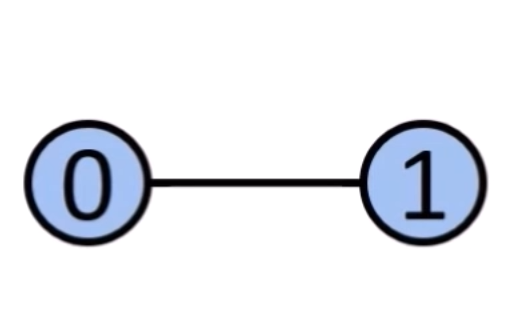
\includegraphics[width=0.4\textwidth]{01.png}
    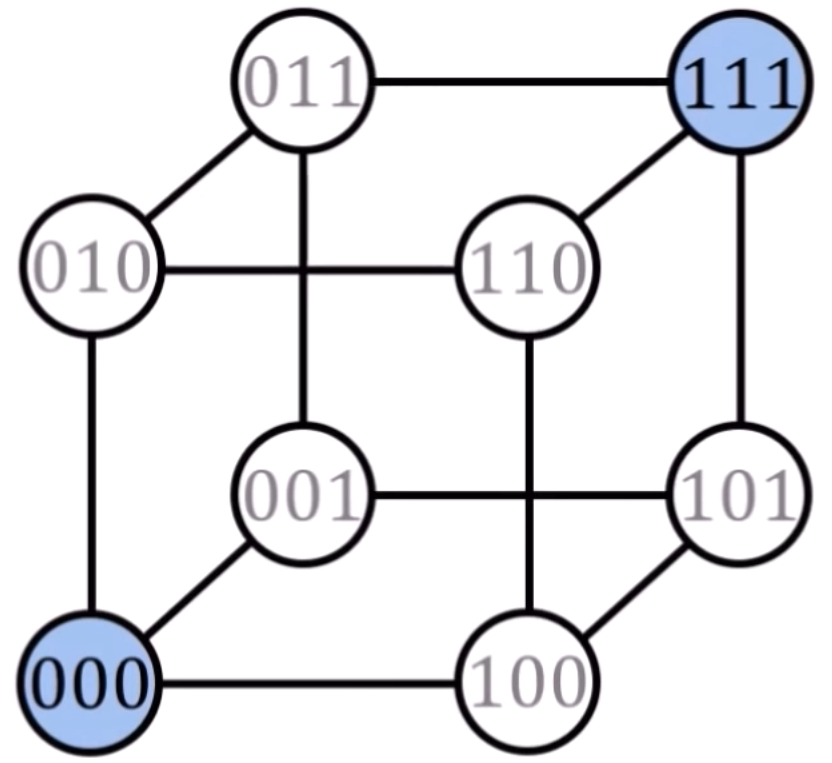
\includegraphics[width=0.4\textwidth]{000-111.png}
\end{frame}


%%%%%%%%%%%%%%%%%%%%%%%%%%%%%%%%%%%%
%%%%%%%%%%%% FIRE CODES %%%%%%%%%%%%
%%%%%%%%%%%%%%%%%%%%%%%%%%%%%%%%%%%%
\section{Fire Codes}
\frame{\sectionpage}


\begin{frame}{Fire Codes}
    \begin{itemize}
        \item Type of burst error correcting code.
        \pause
        \item Appeared originally in Philip Fire's 1959 dissertation, \textit{A class of multiple-error-correcting binary codes for non-independent errors}.
    \end{itemize}
\end{frame}

\begin{frame}{Building a Fire Code}
    \begin{itemize}
        \item Let $p(x)$ be a prime/irreducible polynomial of degree $m$ over $\mathbb{F}_2$.
        \begin{itemize}
            \item An irreducible polynomial cannot be factored into products of non-constant polynomials.
        \end{itemize}
        \pause
        \item Let $\rho$ be the smallest integer such that $p(x) \mid (1 + x^\rho)$. $\rho$ is called the \textit{period}.
        \pause
        \item Let $\ell$ be a positive integer not divisible by $\rho$ with $\ell \le m$.
        \pause
        \item $g(x) = (1 + x^{2\ell - 1})p(x)$ is the generator polynomial for a Fire code.
    \end{itemize}
\end{frame}

\begin{frame}{Example}
    \begin{itemize}
        \item Start with $p(x) = 1 + x + x^3$. (Note: $m = 3$.)
        \pause
        \item We can find $\rho$ with $\rho = 2^m - 1$, so $\rho = 2^3 - 1 = 7$.
        \pause
        \item Select $\ell = 3$. We have $\ell \le m$ and $p \not{\vert} \text{ } (2 \ell - 1)$, so this choice works.
        \pause
        \item Thus,
        \begin{align*}
            g(x)
            & = (1 + x^{2\ell - 1})p(x) \\
            & = (1 + x^5)(1 + x + x^3) \\
            & = 1 + x + x^3 + x^5 + x^6 + x^8
        \end{align*}
    \end{itemize}
\end{frame}

\begin{frame}{Correct codes of length $\le \ell$}
    \begin{thrm}
        Fire codes can correct burst errors of length $\ell$.
    \end{thrm}
    \begin{pf}
        General idea: proof by contradiction of the lemma from before that distinct burst errors must be in distinct cosets.
        \begin{lem}
            $(1 + x^{2\ell - 1})$ and  $p(x)$ (the factors of $g(x)$) are relatively prime.
        \end{lem}
    \end{pf}
\end{frame}

\begin{frame}{Proof}
    \begin{itemize}
            \item Take two \textit{distinct} burst errors with lengths $\ell_1, \ell_2 <  \ell$ represented by
                \begin{align*}
                    a(x) &= 1 + a_1x + a_2x^2 + \cdots + a_{\ell_1 - 2} + x^{\ell_1 - 1} \\
                    b(x) &= 1 + b_1x + b_2x^2 + \cdots + b_{\ell_2 - 2} + x^{\ell_2 - 1}
                \end{align*}
            \pause
            \item These errors could be anywhere, so we write $x^ia(x)$ and $x^jb(x)$ for some $i, j < n$ representing start of error (\textit{WLOG} assume $i < j$).
            \pause
            \item Suppose for contradiction $x^ia(x)$ and $x^jb(x)$ are in the same coset. ($x^ia(x) = x^jb(x) + c$ for some code word $c$)
            \pause
            \item Then their sum, $x^ia(x) + x^jb(x)$, is a polynomial $v(x)$ in the code.
            \pause
            \item Let $q, b$ such that $j - i = q(2\ell - 1) + b$. 
        \end{itemize}
\end{frame}

\begin{frame}{Proof}
    \begin{itemize}
        \item Then
            \begin{align*}
                \onslide<.->{v(x)
                & = x^ia(x) + x^jb(x) \\}
                \onslide<+->{& = x^ia(x) + x^jb(x) + 2x^{b + i}b(x) \\}
                \onslide<+->{& = x^i\big(a(x) + x^bb(x)\big) + x^{b + i}b(x)(1 + x^{q(2\ell - 1)})}
            \end{align*}
        \pause
        \item Because $v(x)$ represents code word, it is divisible by $g(x)$.
        \pause
        \item Because the factors of $g(x)$ are relatively prime, $v(x)$ must  be divisible by $1 + x^{2\ell - 1}$.
        \pause
        \item So $a(x) + x^bb(x)$ is divisible by $1 + x^{2\ell - 1}$ (or is $0$). Let $d(x)$ be the quotient with degree $\delta$.
    \end{itemize}
\end{frame}

\begin{frame}{Proof}
    $$\overbrace{d(x)}^{\delta}\overbrace{(1 + x^{2\ell - 1})}^{2\ell - 1} = \overbrace{a(x)}^{\ell_1 - 1} + \overbrace{x^bb(x)}^{b + \ell_2 - 1}$$
\end{frame}
\begin{frame}{Proof}
    $$\underbrace{\overbrace{d(x)}^{\delta}\overbrace{(x^{2\ell - 1} + 1)}^{2\ell - 1}}_{2\ell - 1 + \delta} = \overbrace{a(x)}^{\ell_1 - 1} + \overbrace{x^bb(x)}^{b + \ell_2 - 1}$$
    \pause
    \begin{alignat*}{2}
        \onslide<+->{&&\ell_1 - 1 &< 2\ell - 1  \\}
        \onslide<+->{&\implies &b + \ell_2 - 1 &= 2\ell - 1 + \delta \\}
        \onslide<+->{&\implies&b &= 2\ell - \ell_2 + \delta \\}
        \onslide<+->{&\implies &b &\ge \ell + \delta \\}
        \onslide<+->{&&&\Downarrow \\ }
        \onslide<.->{&&b > \ell_1 - 1 \text{ }&\text{and } b > \delta}
    \end{alignat*}
\end{frame}


\begin{frame}{Proof}
    $$b > \ell_1 - 1 \text{ and } b > \delta$$
    \begin{itemize}
        \pause
        \item Using $b > \ell_1 - 1$, we know $x^b$ appears in the expansion of $a(x) + x^bb(x)$: 
        \begin{align*}
            1 &+ a_1x + a_2x^2 + \cdots + a_{\ell_1 - 2} + x^{\ell_1 - 1} \\
            &+ x^b(1 + b_1x + b_2x^2 + \cdots + b_{\ell_2 - 2} + x^{\ell_2 - 1})
        \end{align*}
        \pause
        \item Then, using $b > \delta$, we know $d(x)$ does not have $x^b$, so $a(x) + x^bb(x)$ is not divisible by $d(x)$.
        \pause
        \item Recall this means $a(x) + x^bb(x) = 0$.
    \end{itemize}
\end{frame}

\begin{frame}{Proof}
    \begin{align*}
        \onslide<+->{a(x) + x^bb(x) & = 1 + a_1x + a_2x^2 + \cdots + a_{\ell_1 - 2} + x^{\ell_1 - 1} \\}
        \onslide<.->{& \quad+ x^b(1 + b_1x + b_2x^2 + \cdots + b_{\ell_2 - 2} + x^{\ell_2 - 1}) \\}
        \onslide<.->{& = 0 \\}
        \onslide<+->{& \implies b = 0 \quad\quad\quad\quad \text{(remember, we're in } \mathbb{F}_2\text{)}\\}
        \onslide<+->{& \implies a(x) = b(x) \\}
        \onslide<+->{& \implies \text{Contradiction!}}
    \end{align*}
    \pause
    So, if two errors are distinct, they are in different cosets.
\end{frame}

\begin{frame}{Example and Analysis}
    \begin{itemize}
        \item Recall our example of $g(x) = (1 + x^5)(1 + x + x^3)$ with $m = 3$, $\rho = 7$, and $\ell = 3$.
        \pause
        \item Block length $n = \emph{LeastCommonMulitple}(2\ell - 1, p)$.
        \pause
        \begin{itemize}
            \item In this case, $n = \emph{LCM}(5,7) = 35$.
        \end{itemize}
        \pause
        \item Original message length $k = n - m - 2\ell + 1$.
        \pause
        \begin{itemize}
            \item $k = 27$.
            \pause
            \item Would be $29.8$ if it were a Hamming code$^*$.
        \end{itemize}
        \pause
        \item $(35, 27)$ code. Rate gets better with larger blocks.
    \end{itemize}
\end{frame}

\begin{frame}{Not as Good as Reed-Solomon}
  \begin{center}
    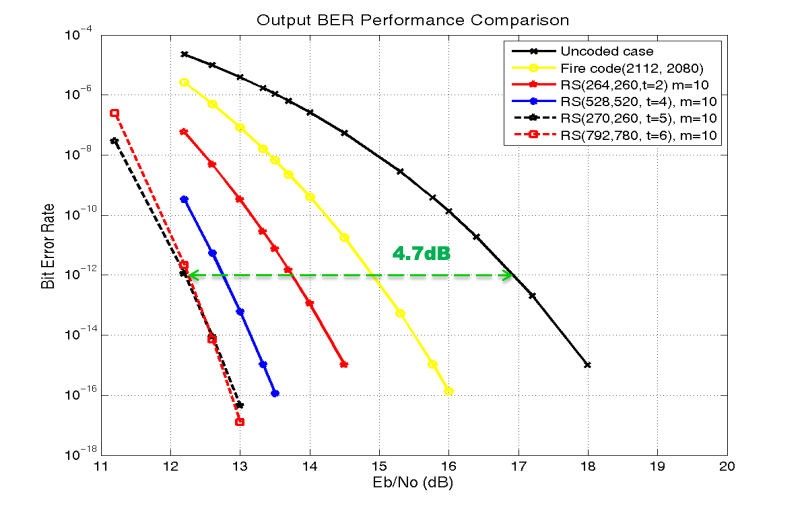
\includegraphics[width=0.85\textwidth]{fire-vs-reed.png}
  \end{center}
\end{frame}

%%%%%%%%%%%%%%%%%%%%%%%%%%%%%%%%%%%%
%%%%%%%%% INTERLEAVED CODES %%%%%%%%
%%%%%%%%%%%%%%%%%%%%%%%%%%%%%%%%%%%%
\section{Interleaved Codes}
\frame{\sectionpage}


\begin{frame}{Interleaved Codes}
    \begin{itemize}
        \item We have many codes that work well, if errors are randomly distributed in our message
        \item But errors are more likely to be spatially correlated \pause
        \item What if we split up the errors, so errors within a burst error are spread out across different words?
    \end{itemize}
\end{frame}


\begin{frame}{Interleaved Codes}
    \begin{itemize}
        \item Built off of codes that are better suited for randomly distributed errors (ex: Hamming Codes) \pause
        \item After encoding the message, but before sending it, we use some bijective function to scramble up the bits (the interleave step) \pause
        \item We send the message, and some burst error occurs \pause
        \item After receiving the message, we descramble the bits (the deinterleave step), sending errors to different code words \pause
        \item We use the underlying code to detect and / or correct errors
    \end{itemize}
\end{frame}


\begin{frame}{Interleaved Codes With a Block Interleaver}
    \begin{itemize}
        \item One way to interleave a message
        \item Organize message as a $M \times N$ matrix: write bits in row major order, read in column major order
        \item Alternatively, write matrix in row major order, transpose the matrix, read the matrix in row major order
    \end{itemize}
    \begin{columns}[c]
    \begin{column}{4cm}
    $x_0 x_1 x_2 x_3 x_4 x_5 x_6 x_7 x_8 \to$
    \end{column}
    \begin{column}{2cm}
    \begin{table}
        \centering
        \begin{tabular}{|c|c|c|}
            \hline 
            $x_0$ & $x_1$ & $x_2$ \\ \hline
            $x_3$ & $x_4$ & $x_5$ \\ \hline
            $x_6$ & $x_7$ & $x_8$ \\ \hline
        \end{tabular}
    \end{table}
    \end{column}
    \begin{column}{5cm}
        $\to x_0 x_3 x_6 x_1 x_4 x_7 x_2 x_5 x_8$
    \end{column}
    \end{columns}
\end{frame}


\begin{frame}{Block Interleaver Example}
    000 \quad 000 \quad 111 \quad 000 \pause $\to$ \\
    \begin{table}
        \centering
        \begin{tabular}{|c|c|c|}
            \hline 
            0 & \err{0} & \lgreen{0} \\ \hline
            0 & \err{0} & \blu{0} \\ \hline
            1 & \lgreen{1} & \blu{1} \\ \hline
            \err{0} & \lgreen{0} & \blu{0} \\ \hline
        \end{tabular}
    \end{table} \pause

    $\to$ 001 \quad \err{000} \quad \lgreen{100} \quad \blu{010}
\end{frame}


\begin{frame}{Block Interleaver Example}
    001000100010 + 00\err{111}0000000 = 00\err{011}0100010 \pause $\to$ \\

    \begin{table}
        \centering
        \begin{tabular}{|c|c|c|}
            \hline 
            0 & \err{1} & 0 \\ \hline
            0 & 0 & 0 \\ \hline
            \err{0} & 1 & 1 \\ \hline
            \err{1} & 0 & 0 \\ \hline
        \end{tabular}
    \end{table} \pause

    $\to$ 0\err{1}0 \quad 000 \quad \err{0}11 \quad \err{1}00
\end{frame}


\begin{frame}{Block Interleaver Analysis}
    \begin{itemize}
        \item Take a burst error of length $\ell$
        \item After interleaving, the distance between consecutive errors becomes $M$
        \item We need a burst error of length $M \cdot \ell + 1$ to get $\ell + 1$ consecutive errors in the output \pause
        \item Thus, a code that can correct $t$ errors can correct $M \cdot t$ burst errors.
    \end{itemize}
\end{frame}


\begin{frame}{Block Interleaver Analysis}
    \begin{itemize}
        \item Block Interleaver takes up $M \cdot N$ space
        \item We can measure its efficiency by comparing how many errors can occur until it fails and how much space it takes up
        \item efficiency $= \frac {M \cdot t + 1}{M \cdot N} \approx \frac {M \cdot t}{M \cdot N} = \frac t N$
    \end{itemize}
\end{frame}


\begin{frame}{Block Interleaver Analysis}
    \begin{itemize}
        \item One major downside: we need to read almost the entire transmitted message before we can start deinterleaving it and running error detection / correction on it \pause
        \item Not necessarily as good for data streams \pause
        \item Possible solution: apply interleaving to blocks of data at a time \pause
        \item Possible issue with this solution: how do we know when blocks start / end in the data stream?
    \end{itemize}
\end{frame}


\begin{frame}{Interleaved Codes With a Convolution Interleaver}
    \begin{itemize}
        \item A different interleaving approach
        \item Sometimes called a cross interleaver
        \item Interleave by putting consecutive elements into consequtive queues of varying lengths
    \end{itemize}

    \bigskip

    \begin{columns}[c]
    \begin{column}{3cm}
        $\ldots x_3 x_4 x_5 x_6 x_7 x_8 \ldots \to$
    \end{column}
    \hfill
    \begin{column}{5cm}
    \begin{table}
        \centering
        \begin{tabular}{c|c|c|c|c}
            \hline
            & $x_6$ \\ \hline
            & $x_7$ & $x_4$ \\ \hline
            & $x_8$ & $x_5$ & $x_2$ & \\ \hline
        \end{tabular}
    \end{table}
    \end{column}
    \hfill
    \begin{column}{5cm}
        $\to \ldots x_6 x_4 x_2 x_9 x_7 x_5 \ldots$
    \end{column}
    \end{columns}
\end{frame}


\begin{frame}{Convolution Interleaver: Another Approach}
    \begin{itemize}
        \item Write the message as a matrix and shift columns down by varying amounts.
    \end{itemize}

    \begin{columns}[c]
    \begin{column}{1cm}
        $x_0 x_1 x_2 x_3 x_4 x_5 x_6 x_7 x_8 \to$
    \end{column}
    \hfill
    \begin{column}{5cm}
    \begin{table}
        \centering
        \begin{tabular}{|c|c|c|}
            \hline
            $x_0$ & $x_1$ & $x_2$ \\ \hline
            $x_3$ & $x_4$ & $x_5$ \\ \hline
            $x_6$ & $x_7$ & $x_8$ \\ \hline
        \end{tabular}
    \end{table}
    \end{column}
    \end{columns}
\end{frame}


\begin{frame}{Convolution Interleaver: Another Approach}
    \begin{itemize}
        \item Write the message as a matrix in row major order and shift columns down by varying amounts.
    \end{itemize}

    \begin{columns}[c]
    \begin{column}{1cm}
        $x_0 x_1 x_2 x_3 x_4 x_5 x_6 x_7 x_8 \to$
    \end{column}
    \hfill
    \begin{column}{5cm}
    \begin{table}
        \centering
        \begin{tabular}{|c|c|c|}
            \hline
            $x_0$ &   &   \\ \hline
            $x_3$ & $x_1$ &   \\ \hline
            $x_6$ & $x_4$ & $x_2$ \\ \hline
              & $x_7$ & $x_5$ \\ \hline
              &   & $x_8$ \\ \hline
        \end{tabular}
    \end{table}
    \end{column}
    \end{columns}

    \bigskip
    
    $\to \ldots x_6 x_4 x_2 \ldots$
\end{frame}


\begin{frame}{Convolution Interleaver: Deinterleaving}
    \begin{columns}[c]
    \begin{column}{4cm}
        $\ldots x_6 x_4 x_2 x_9 x_7 x_5 \ldots \to$
    \end{column}
    \hfill
    \begin{column}{3cm}
    \begin{table}
        \centering
        \begin{tabular}{c|c|c|c|c}
            \hline
            & $x_9$ & $x_6$ & $x_3$ & \\ \hline
            & $x_7$ & $x_4$ \\ \hline
            & $x_5$ \\ \hline
        \end{tabular}
    \end{table}
    \end{column}
    \hfill
    \begin{column}{5cm}
        $\to \ldots x_3 x_4 x_5 x_6 x_7 x_8 \ldots$
    \end{column}
    \end{columns}
\end{frame}


\begin{frame}{Convolution Interleaver: Deinterleaving}
    \begin{columns}[c]
    \begin{column}{1cm}
        $\ldots x_6 x_4 x_2 \ldots \to$
    \end{column}
    \begin{column}{5cm}
    \begin{table}
        \centering
        \begin{tabular}{|c|c|c|}
            \hline
            $x_0$ &   &   \\ \hline
            $x_3$ & $x_1$ &   \\ \hline
            $x_6$ & $x_4$ & $x_2$ \\ \hline
              & $x_7$ & $x_5$ \\ \hline
              &   & $x_8$ \\ \hline
        \end{tabular}
    \end{table}
    \end{column}
    \end{columns}

    \begin{columns}[c]
    \begin{column}{1cm}
    \begin{table}
        \centering
        \begin{tabular}{|c|c|c|}
            \hline
            $x_0$ & $x_1$ & $x_2$ \\ \hline
            $x_3$ & $x_4$ & $x_5$ \\ \hline
            $x_6$ & $x_7$ & $x_8$ \\ \hline
        \end{tabular}
    \end{table}
    \end{column}
    \hfill
    \begin{column}{5cm}
        $\to x_0 x_1 x_2 x_3 x_4 x_5 x_6 x_7 x_8$
    \end{column}
    \end{columns}
\end{frame}


\begin{frame}{Convolution Interleaver Example}
    000 \quad 000 \quad 111 \quad 000 \pause $\to$ \\
    \begin{table}
        \centering
        \begin{tabular}{|c|c|c|}
            \hline 
            0 & 0 & 0 \\ \hline
            0 & 0 & 0 \\ \hline
            1 & 1 & 1 \\ \hline
            0 & 0 & 0 \\ \hline
        \end{tabular}
    \end{table} \pause

    $\to$

    \begin{table}
        \centering
        \begin{tabular}{|c|c|c|}
            \hline 
            0 & - & - \\ \hline
            0 & 0 & - \\ \hline
            1 & 0 & 0 \\ \hline
            0 & 1 & 0 \\ \hline
            - & 0 & 1 \\ \hline
            - & - & 0 \\ \hline
        \end{tabular}
    \end{table} \pause

    $\to$ 0\_\_00\_100010\_01\_\_0
\end{frame}


\begin{frame}{Convolution Interleaver Example}
    \begin{align*}
    0\_\_00\_100010\_01\_\_0 &+ 0\_\_0\err{1\_1}00\err{1}00\_00\_\_0 \\
    &= 0\_\_0\err{1\_0}00\err{1}10\_01\_\_0
    \end{align*} \pause

    $\to$

    \begin{table}
        \centering
        \begin{tabular}{|c|c|c|}
            \hline 
            0 & - & - \\ \hline
            0 & \err{1} & \err{-} \\ \hline
            \err{0} & 0 & 0 \\ \hline
            \err{1} & 1 & 0 \\ \hline
            - & 0 & 1 \\ \hline
            - & - & 0 \\ \hline
        \end{tabular}
    \end{table}
\end{frame}


\begin{frame}{Convolution Interleaver Example}
    $\to$
    
    \begin{table}
        \centering
        \begin{tabular}{|c|c|c|}
            \hline 
            0 & \err{1} & 0 \\ \hline
            0 & 0 & 0 \\ \hline
            \err{0} & 1 & 1 \\ \hline
            \err{1} & 0 & 0 \\ \hline
        \end{tabular}
    \end{table} \pause

    $\to$ 0\err{1}0 \quad 000 \quad \err{0}11 \quad \err{1}00
\end{frame}


\begin{frame}{Convolution Interleaver Analysis}
    \begin{itemize}
        \item Difference between consecutive errors becomes $N + 1$
        \item We can correct up to $(N + 1)(t - 1)$ errors
        \item Takes up $0 + 1 + \ldots + (N - 1) = \frac {N (N - 1)} 2$ space \pause
        \item We no longer have to read nearly the entire message to start decoding
    \end{itemize}
\end{frame}


\begin{frame}{Convolution Interleaver Analysis}
    \begin{itemize}
        \item We can measure its efficiency by comparing how many errors can occur until it fails and how much space it takes up
        \item efficiency $= \frac {(N + 1)(t - 1) + 1}{\frac {N (N - 1)} 2} \approx \frac {N \cdot t}{\frac {N^2} 2} = \frac {2t} N$ \pause
        \item Notice that the efficiency for the convolution interleaver is approximately twice as good as that of the block interleaver (which had efficiency $= \frac t N$)
    \end{itemize}
\end{frame}


\section{Unary Codes}
\frame{\sectionpage}


\begin{frame}{Unary Codes}
    \begin{center}
        \pause
        $000000$
        \pause
        $\xrightarrow{\text{error of }0{\color{red}0}0{\color{red}00}0}$
        \pause
        $0{\color{red}0}0{\color{red}00}0$
        \pause 
        $\rightarrow 000000$
    \end{center}
\end{frame}

% Quotes are fun, find some to use!
\font\eightss=cmssq8
\font\eightssi=cmssqi8
\newcommand\quoteAuthorDate[3]{\begingroup
  \baselineskip 10pt
  \parfillskip 0pt
  \interlinepenalty 10000 % not needed in example
  \leftskip 0pt plus 40pc minus \parindent
  \let\rm=\eightss
  \let\sl=\eightssi
  \everypar{\sl}#1\par
  \nobreak\smallskip
  \noindent\rm--- #2\unskip\enspace(#3)\par
  \endgroup}
% If someone can figure out how to horizontally center this and make the text bigger that'd be cool
\begin{frame}
    \begin{center}
        \item \quoteAuthorDate{Information is the resolution of uncertainty.}{Claude Shannon}{\color{sigma@mainblue} 1948}
    \end{center}
\end{frame}

% Remove this slide if you came up with all the material yourself
\begin{frame}{Bibliography}
    \bibliography{refs}
    \bibliographystyle{alpha}
    Moon, Todd K. \textit{Error Correction Coding: Mathematical Methods and Algorithms.} John Wiley \& Sons, Inc., 2005. 
\end{frame}

\end{document}